\documentclass[aspectratio=169, 11pt]{beamer}
% ============================================================================
% Preambulo compartido para presentaciones Beamer
% Estadistica 2026-II - Pontificia Universidad Javeriana
% Incluir con: % ============================================================================
% Preambulo compartido para presentaciones Beamer
% Estadistica 2026-II - Pontificia Universidad Javeriana
% Incluir con: % ============================================================================
% Preambulo compartido para presentaciones Beamer
% Estadistica 2026-II - Pontificia Universidad Javeriana
% Incluir con: \input{../preambulo_beamer.tex} despues de \documentclass
% ============================================================================

\usepackage[T1]{fontenc}
\usepackage[utf8]{inputenc}
\usepackage[spanish]{babel}
\usepackage{amsmath, amssymb, amsfonts}
\usepackage{booktabs}
\usepackage{graphicx}
\usepackage{tikz}
\usetikzlibrary{shapes.geometric, positioning, arrows.meta, calc}
\usepackage{pgfplots}
\pgfplotsset{compat=1.18}
\usepackage{listings}
\usepackage{xcolor}
\usepackage{hyperref}
\usepackage{multicol}


% --- Tema Beamer (minimalista) ---
\usetheme{default}
\usecolortheme{default}
\usefonttheme{default}
\setbeamertemplate{navigation symbols}{}
\setbeamertemplate{caption}[numbered]
\setbeamertemplate{footline}{%
  \hfill\usebeamerfont{footline}\insertframenumber/\inserttotalframenumber\hspace{1em}\vspace{0.5em}%
}
\setbeamertemplate{itemize items}[circle]
\setbeamertemplate{enumerate items}[default]

% --- Colores institucionales (sutiles) ---
\definecolor{javeriana}{RGB}{0, 62, 105}
\definecolor{javerianalight}{RGB}{0, 105, 170}
\definecolor{codigobg}{RGB}{245, 245, 245}
\definecolor{codigofg}{RGB}{40, 40, 40}
\definecolor{comentario}{RGB}{100, 100, 100}
\definecolor{keyword}{RGB}{0, 100, 150}
\definecolor{string}{RGB}{180, 60, 30}

\setbeamercolor{title}{fg=javeriana}
\setbeamercolor{frametitle}{fg=javeriana}
\setbeamercolor{structure}{fg=javeriana}
\setbeamercolor{block title}{fg=white, bg=javeriana!75}
\setbeamercolor{block body}{bg=javeriana!5}
\setbeamercolor{block title alerted}{fg=white, bg=red!70!black}
\setbeamercolor{block body alerted}{bg=red!5}
\setbeamercolor{block title example}{fg=white, bg=green!40!black}
\setbeamercolor{block body example}{bg=green!5}
\setbeamercolor{item}{fg=javeriana}

\setbeamerfont{title}{series=\bfseries, size=\Large}
\setbeamerfont{frametitle}{series=\bfseries}

% --- Configuracion de listings para R ---
\lstset{
  language=R,
  basicstyle=\ttfamily\footnotesize,
  backgroundcolor=\color{codigobg},
  commentstyle=\color{comentario}\itshape,
  keywordstyle=\color{keyword}\bfseries,
  stringstyle=\color{string},
  numbers=none,
  frame=single,
  rulecolor=\color{javeriana!30},
  breaklines=true,
  showstringspaces=false,
  columns=flexible,
  morekeywords={library, ggplot, aes, geom_histogram, geom_boxplot,
    geom_point, geom_smooth, geom_density, geom_bar, geom_line,
    geom_vline, geom_hline, geom_errorbar, labs, theme_minimal,
    facet_wrap, scale_fill_manual, scale_color_manual,
    summarise, group_by, filter, mutate, select, arrange,
    read.csv, head, str, summary, mean, median, sd, var, cor,
    lm, t.test, chisq.test, wilcox.test, kruskal.test, aov,
    pnorm, qnorm, dnorm, rnorm, qt, pt, qchisq, pchisq, qf, pf,
    confint, coeftest, vcovHC, bptest, vif, cooks.distance,
    TukeyHSD, table, prop.table}
}

% --- Comandos personalizados ---
\newcommand{\R}{\texttt{R}}
\newcommand{\code}[1]{\texttt{\footnotesize #1}}
\newcommand{\variable}[1]{\texttt{#1}}
\newcommand{\paquete}[1]{\texttt{#1}}

% --- Informacion del curso ---
\institute{Pontificia Universidad Javeriana\\
  Facultad de Ciencias Económicas y Administrativas}
\date{2026-II}
 despues de \documentclass
% ============================================================================

\usepackage[T1]{fontenc}
\usepackage[utf8]{inputenc}
\usepackage[spanish]{babel}
\usepackage{amsmath, amssymb, amsfonts}
\usepackage{booktabs}
\usepackage{graphicx}
\usepackage{tikz}
\usetikzlibrary{shapes.geometric, positioning, arrows.meta, calc}
\usepackage{pgfplots}
\pgfplotsset{compat=1.18}
\usepackage{listings}
\usepackage{xcolor}
\usepackage{hyperref}
\usepackage{multicol}


% --- Tema Beamer (minimalista) ---
\usetheme{default}
\usecolortheme{default}
\usefonttheme{default}
\setbeamertemplate{navigation symbols}{}
\setbeamertemplate{caption}[numbered]
\setbeamertemplate{footline}{%
  \hfill\usebeamerfont{footline}\insertframenumber/\inserttotalframenumber\hspace{1em}\vspace{0.5em}%
}
\setbeamertemplate{itemize items}[circle]
\setbeamertemplate{enumerate items}[default]

% --- Colores institucionales (sutiles) ---
\definecolor{javeriana}{RGB}{0, 62, 105}
\definecolor{javerianalight}{RGB}{0, 105, 170}
\definecolor{codigobg}{RGB}{245, 245, 245}
\definecolor{codigofg}{RGB}{40, 40, 40}
\definecolor{comentario}{RGB}{100, 100, 100}
\definecolor{keyword}{RGB}{0, 100, 150}
\definecolor{string}{RGB}{180, 60, 30}

\setbeamercolor{title}{fg=javeriana}
\setbeamercolor{frametitle}{fg=javeriana}
\setbeamercolor{structure}{fg=javeriana}
\setbeamercolor{block title}{fg=white, bg=javeriana!75}
\setbeamercolor{block body}{bg=javeriana!5}
\setbeamercolor{block title alerted}{fg=white, bg=red!70!black}
\setbeamercolor{block body alerted}{bg=red!5}
\setbeamercolor{block title example}{fg=white, bg=green!40!black}
\setbeamercolor{block body example}{bg=green!5}
\setbeamercolor{item}{fg=javeriana}

\setbeamerfont{title}{series=\bfseries, size=\Large}
\setbeamerfont{frametitle}{series=\bfseries}

% --- Configuracion de listings para R ---
\lstset{
  language=R,
  basicstyle=\ttfamily\footnotesize,
  backgroundcolor=\color{codigobg},
  commentstyle=\color{comentario}\itshape,
  keywordstyle=\color{keyword}\bfseries,
  stringstyle=\color{string},
  numbers=none,
  frame=single,
  rulecolor=\color{javeriana!30},
  breaklines=true,
  showstringspaces=false,
  columns=flexible,
  morekeywords={library, ggplot, aes, geom_histogram, geom_boxplot,
    geom_point, geom_smooth, geom_density, geom_bar, geom_line,
    geom_vline, geom_hline, geom_errorbar, labs, theme_minimal,
    facet_wrap, scale_fill_manual, scale_color_manual,
    summarise, group_by, filter, mutate, select, arrange,
    read.csv, head, str, summary, mean, median, sd, var, cor,
    lm, t.test, chisq.test, wilcox.test, kruskal.test, aov,
    pnorm, qnorm, dnorm, rnorm, qt, pt, qchisq, pchisq, qf, pf,
    confint, coeftest, vcovHC, bptest, vif, cooks.distance,
    TukeyHSD, table, prop.table}
}

% --- Comandos personalizados ---
\newcommand{\R}{\texttt{R}}
\newcommand{\code}[1]{\texttt{\footnotesize #1}}
\newcommand{\variable}[1]{\texttt{#1}}
\newcommand{\paquete}[1]{\texttt{#1}}

% --- Informacion del curso ---
\institute{Pontificia Universidad Javeriana\\
  Facultad de Ciencias Económicas y Administrativas}
\date{2026-II}
 despues de \documentclass
% ============================================================================

\usepackage[T1]{fontenc}
\usepackage[utf8]{inputenc}
\usepackage[spanish]{babel}
\usepackage{amsmath, amssymb, amsfonts}
\usepackage{booktabs}
\usepackage{graphicx}
\usepackage{tikz}
\usetikzlibrary{shapes.geometric, positioning, arrows.meta, calc}
\usepackage{pgfplots}
\pgfplotsset{compat=1.18}
\usepackage{listings}
\usepackage{xcolor}
\usepackage{hyperref}
\usepackage{multicol}


% --- Tema Beamer (minimalista) ---
\usetheme{default}
\usecolortheme{default}
\usefonttheme{default}
\setbeamertemplate{navigation symbols}{}
\setbeamertemplate{caption}[numbered]
\setbeamertemplate{footline}{%
  \hfill\usebeamerfont{footline}\insertframenumber/\inserttotalframenumber\hspace{1em}\vspace{0.5em}%
}
\setbeamertemplate{itemize items}[circle]
\setbeamertemplate{enumerate items}[default]

% --- Colores institucionales (sutiles) ---
\definecolor{javeriana}{RGB}{0, 62, 105}
\definecolor{javerianalight}{RGB}{0, 105, 170}
\definecolor{codigobg}{RGB}{245, 245, 245}
\definecolor{codigofg}{RGB}{40, 40, 40}
\definecolor{comentario}{RGB}{100, 100, 100}
\definecolor{keyword}{RGB}{0, 100, 150}
\definecolor{string}{RGB}{180, 60, 30}

\setbeamercolor{title}{fg=javeriana}
\setbeamercolor{frametitle}{fg=javeriana}
\setbeamercolor{structure}{fg=javeriana}
\setbeamercolor{block title}{fg=white, bg=javeriana!75}
\setbeamercolor{block body}{bg=javeriana!5}
\setbeamercolor{block title alerted}{fg=white, bg=red!70!black}
\setbeamercolor{block body alerted}{bg=red!5}
\setbeamercolor{block title example}{fg=white, bg=green!40!black}
\setbeamercolor{block body example}{bg=green!5}
\setbeamercolor{item}{fg=javeriana}

\setbeamerfont{title}{series=\bfseries, size=\Large}
\setbeamerfont{frametitle}{series=\bfseries}

% --- Configuracion de listings para R ---
\lstset{
  language=R,
  basicstyle=\ttfamily\footnotesize,
  backgroundcolor=\color{codigobg},
  commentstyle=\color{comentario}\itshape,
  keywordstyle=\color{keyword}\bfseries,
  stringstyle=\color{string},
  numbers=none,
  frame=single,
  rulecolor=\color{javeriana!30},
  breaklines=true,
  showstringspaces=false,
  columns=flexible,
  morekeywords={library, ggplot, aes, geom_histogram, geom_boxplot,
    geom_point, geom_smooth, geom_density, geom_bar, geom_line,
    geom_vline, geom_hline, geom_errorbar, labs, theme_minimal,
    facet_wrap, scale_fill_manual, scale_color_manual,
    summarise, group_by, filter, mutate, select, arrange,
    read.csv, head, str, summary, mean, median, sd, var, cor,
    lm, t.test, chisq.test, wilcox.test, kruskal.test, aov,
    pnorm, qnorm, dnorm, rnorm, qt, pt, qchisq, pchisq, qf, pf,
    confint, coeftest, vcovHC, bptest, vif, cooks.distance,
    TukeyHSD, table, prop.table}
}

% --- Comandos personalizados ---
\newcommand{\R}{\texttt{R}}
\newcommand{\code}[1]{\texttt{\footnotesize #1}}
\newcommand{\variable}[1]{\texttt{#1}}
\newcommand{\paquete}[1]{\texttt{#1}}

% --- Informacion del curso ---
\institute{Pontificia Universidad Javeriana\\
  Facultad de Ciencias Económicas y Administrativas}
\date{2026-II}

\usepackage{qrcode}
\usepackage{cancel}
\title{Sesiones 8--9: Chi-Cuadrado y Regresión Lineal Simple}
\subtitle{Pruebas categóricas + introducción a OLS}
\author{Prof.\ Jaime Polanco Jiménez}
\date{Vie 16 oct 2026}

\begin{document}

\begin{frame}
\titlepage
\end{frame}

\begin{frame}{Agenda}
\tiny 
\tableofcontents
\end{frame}

% ============================================================================

\section{CHAEA: estilos de aprendizaje del salón}
% ============================================================================

\begin{frame}{Resultado CHAEA: distribución del salón}
\begin{center}
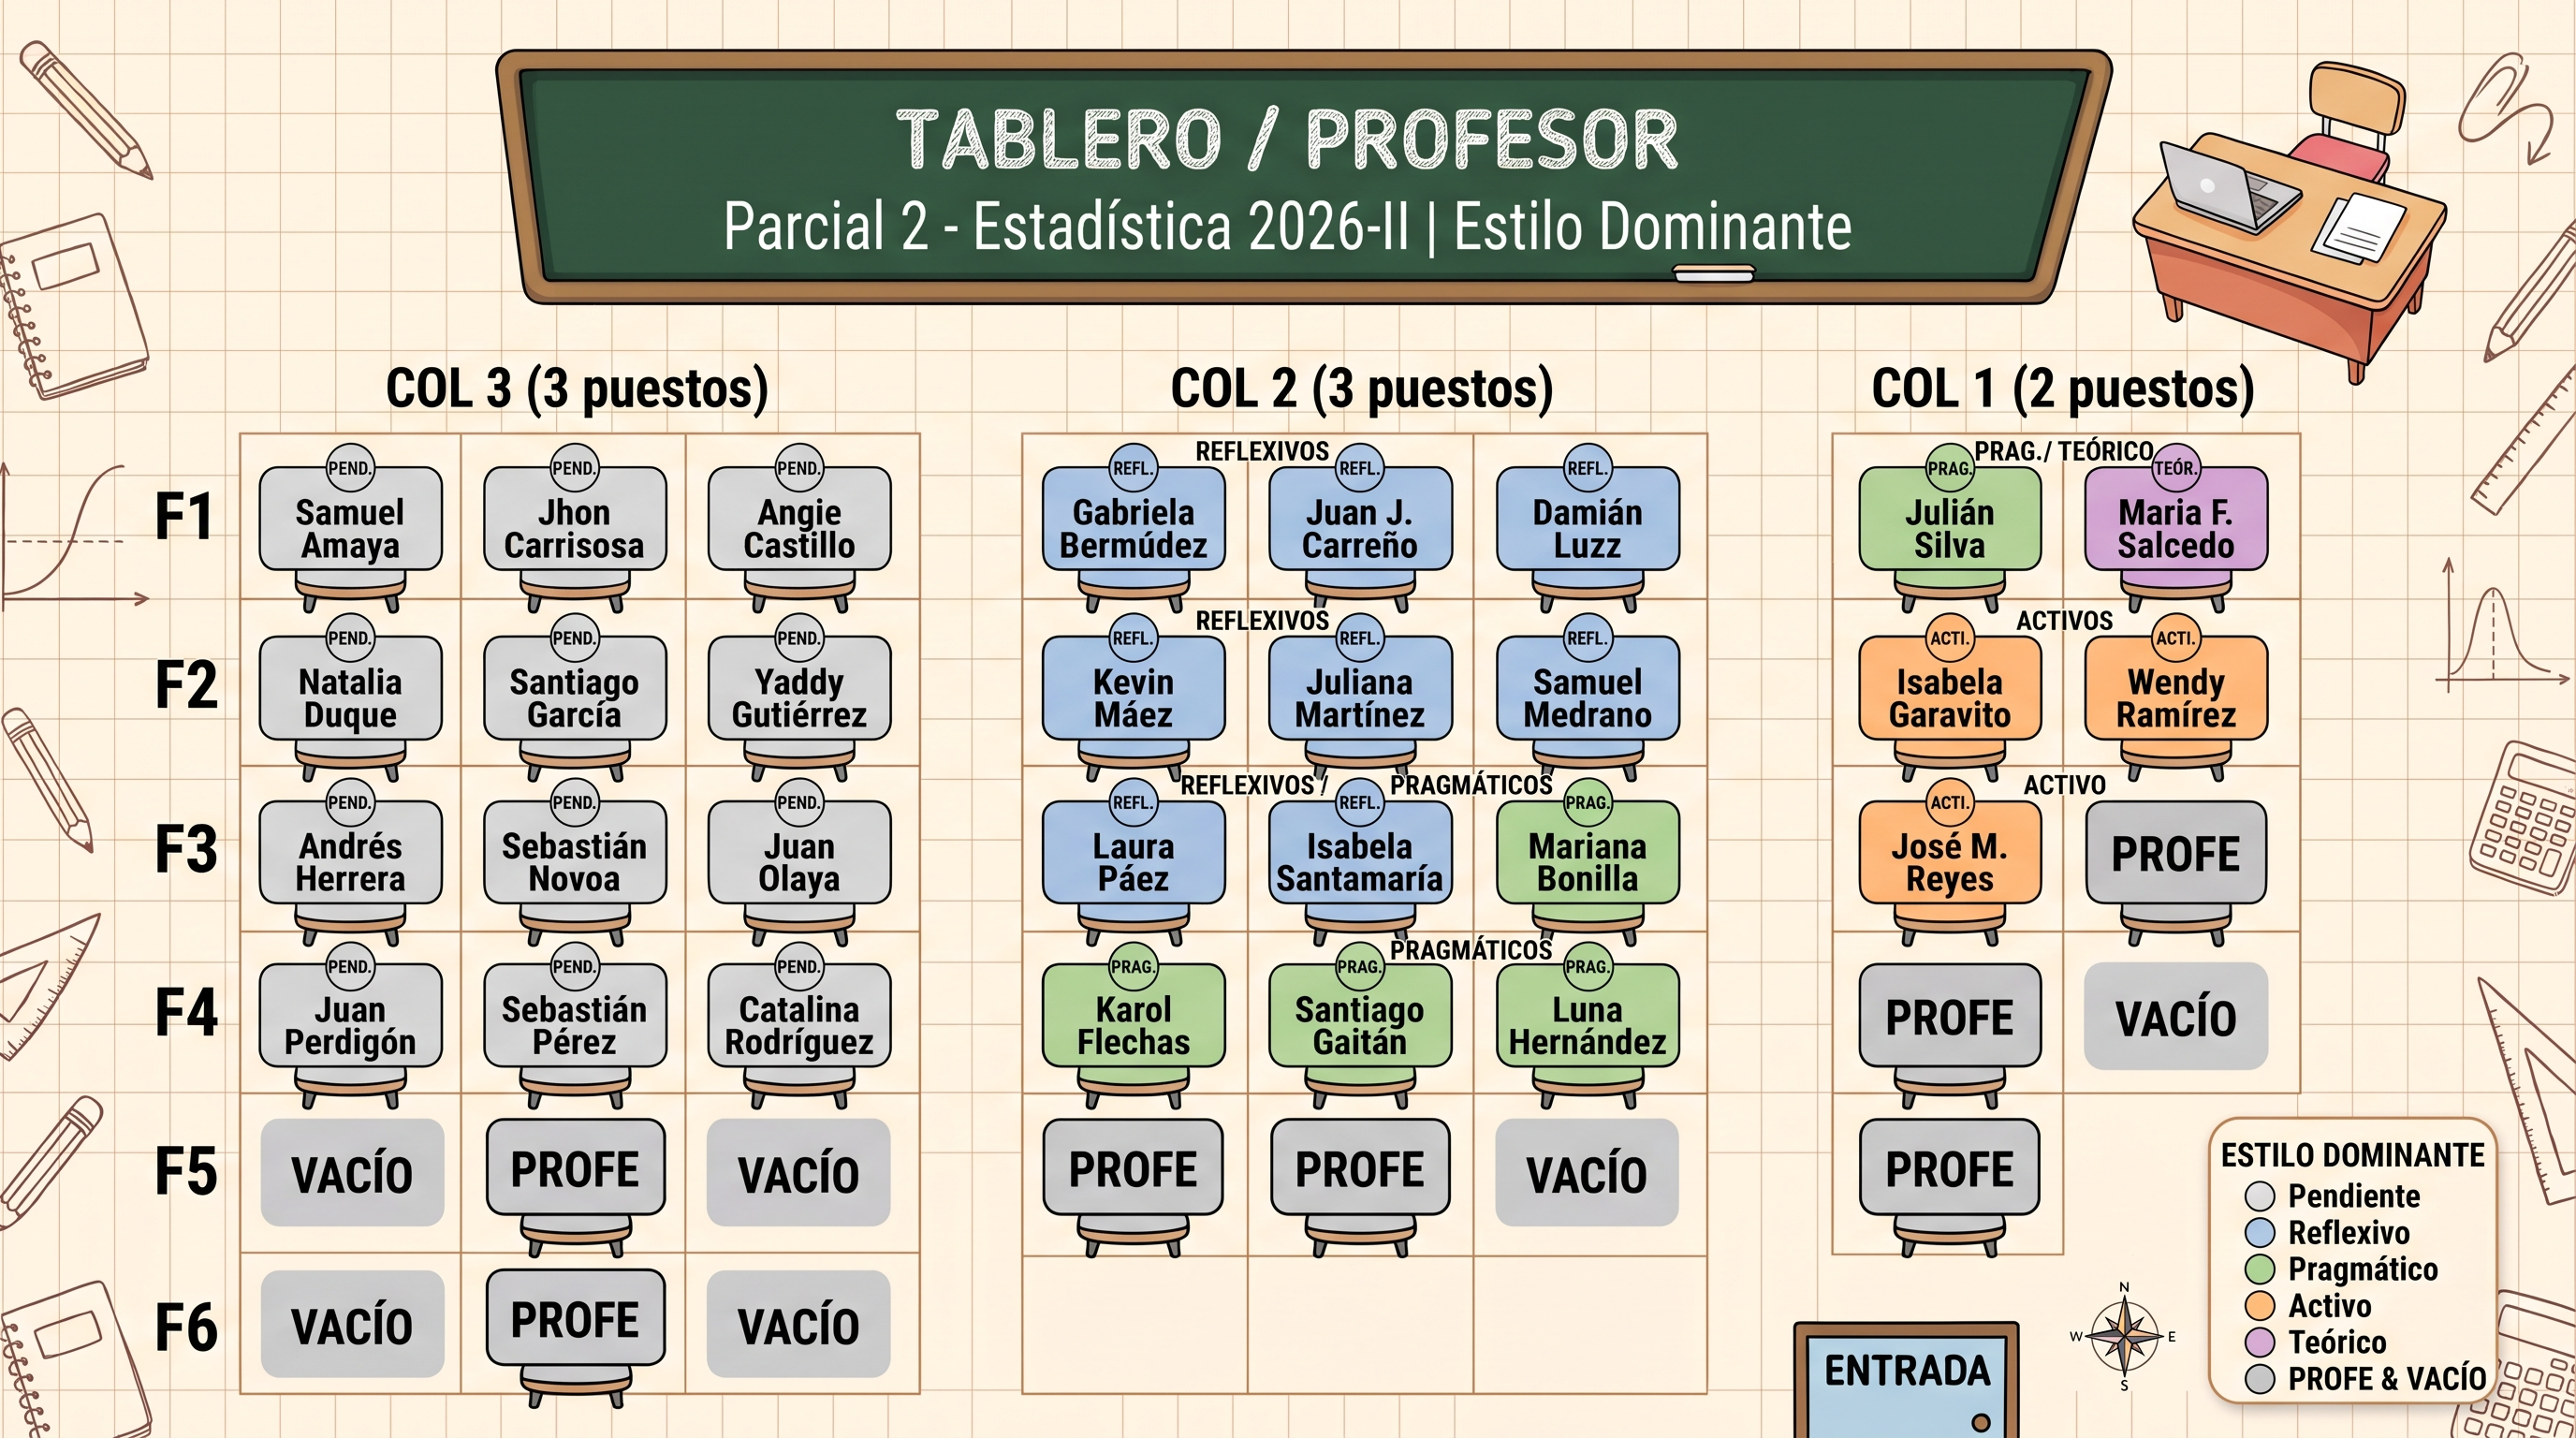
\includegraphics[width=\textwidth,height=0.78\textheight,keepaspectratio]{chaea_distribucion_salon.jpeg}
\end{center}
\end{frame}

\begin{frame}{¿Qué es el CHAEA?}
\small
El \textbf{CHAEA} (Cuestionario Honey-Alonso de Estilos de Aprendizaje) es un test de 80 afirmaciones que identifica cómo prefieren aprender y procesar información.

Se basa en el modelo de Peter Honey y Alan Mumford, y clasifica en \textbf{4 estilos}:

\vspace{0.2cm}
\begin{columns}[T]
\column{0.48\textwidth}
\begin{block}{\textcolor{black}{1. Activo}}
\footnotesize
\textbf{Perfil:} Espontáneos, entusiastas, arriesgados. Actúan primero, piensan después.\\[2pt]
\textbf{Prefieren:} Novedades, retos, trabajo en grupo.\\[2pt]
\textbf{Evitan:} Trabajos largos y monótonos.
\end{block}

\column{0.48\textwidth}
\begin{block}{\textcolor{black}{2. Reflexivo}}
\footnotesize
\textbf{Perfil:} Observadores, analíticos, cautelosos. Consideran todas las opciones antes de decidir.\\[2pt]
\textbf{Prefieren:} Recopilar datos, analizar despacio, tiempo para pensar.\\[2pt]
\textbf{Evitan:} Presión de tiempo, acción rápida.
\end{block}
\end{columns}
\end{frame}

\begin{frame}{Estilos CHAEA (cont.)}
\small
\begin{columns}[T]
\column{0.48\textwidth}
\begin{block}{\textcolor{black}{3. Teórico}}
\footnotesize
\textbf{Perfil:} Buscan racionalidad, lógica y sistemas estructurados. Integran hechos en teorías coherentes.\\[2pt]
\textbf{Prefieren:} Modelos, conceptos, pensar de forma secuencial y metódica.\\[2pt]
\textbf{Evitan:} Ambigüedad, falta de fundamento lógico.
\end{block}

\column{0.48\textwidth}
\begin{block}{\textcolor{black}{4. Pragmático}}
\footnotesize
\textbf{Perfil:} Prácticos, directos, realistas. Les gusta comprobar si las ideas funcionan.\\[2pt]
\textbf{Prefieren:} Aplicar lo aprendido, resolver problemas concretos, ver utilidad práctica.\\[2pt]
\textbf{Evitan:} Teorías sin aplicación clara.
\end{block}
\end{columns}

\vspace{0.3cm}
\begin{alertblock}{¿Por qué nos importa hoy?}
\small Usaremos los resultados del salón como datos categóricos para practicar $\chi^2$: ¿el estilo dominante es independiente del grupo?
\end{alertblock}
\end{frame}

\begin{frame}{Resultado CHAEA: resumen numérico}
\small
De los 29 estudiantes, 17 completaron el test. Distribución de estilos dominantes:

\vspace{0.2cm}
\begin{center}
\begin{tabular}{lcccc}
\toprule
\textbf{Estilo} & \textbf{Frecuencia} & \textbf{Proporción} & \textbf{Mujeres} & \textbf{Hombres} \\
\midrule
\textcolor{green!50!black}{Reflexivo} & 8 & 47.1\% & 4 & 4 \\
\textcolor{orange!80!black}{Pragmático} & 5 & 29.4\% & 3 & 2 \\
\textcolor{blue!70}{Activo} & 3 & 17.6\% & 2 & 1 \\
\textcolor{purple}{Teórico} & 1 & 5.9\% & 1 & 0 \\
\midrule
\textbf{Total} & \textbf{17} & 100\% & 10 & 7 \\
\bottomrule
\end{tabular}
\end{center}

\vspace{0.2cm}
\begin{alertblock}{Pregunta para hoy}
¿El estilo dominante es independiente del género? ¿La distribución es uniforme? Estas son preguntas que responderemos con $\chi^2$.
\end{alertblock}
\end{frame}

% ============================================================================
\section{Repaso completo: de los datos a la decisión}
% ============================================================================

\begin{frame}{}
\vfill
\centering
{\Large\textbf{Repaso: Todo el Pipeline Paso a Paso}}\\[1em]
{\normalsize Un solo ejemplo con 10 personas que recorre \alert{todo} lo que hemos aprendido}\\[0.5em]
{\small S01 $\to$ S02 $\to$ S03 $\to$ S04 $\to$ S06 $\to$ S07 $\to$ \textbf{Hoy}}
\vfill
\end{frame}

% --- PASO 1: Los datos ---
\begin{frame}{Paso 1: Los datos (S01)}
\small
Un investigador quiere probar el estereotipo: ``\textit{los hombres son mejores que las mujeres en matemáticas}.''

\vspace{0.2cm}
Toma una muestra de 10 estudiantes (5~hombres, 5~mujeres) y registra su nota en un examen de matemáticas (sobre 100):

\vspace{0.3cm}
\begin{center}
\begin{tabular}{lccccc|c}
\toprule
& Est.\ 1 & Est.\ 2 & Est.\ 3 & Est.\ 4 & Est.\ 5 & $\bar{x}$ \\
\midrule
\textbf{Hombres} & 82 & 78 & 91 & 85 & 74 & \textbf{82.0} \\
\textbf{Mujeres} & 76 & 80 & 72 & 85 & 77 & \textbf{78.0} \\
\bottomrule
\end{tabular}
\end{center}

\vspace{0.3cm}
\begin{alertblock}{Pregunta central}
Los hombres sacaron 4 puntos más en promedio. ¿Eso es evidencia de que son ``mejores'', o es solo \textbf{suerte muestral}?
\end{alertblock}
\end{frame}

% --- PASO 2: Descriptivos ---
\begin{frame}{Paso 2: Estadísticos descriptivos (S01)}
\small
\textbf{Hombres} ($\bar{x}_H = 82.0$):
\begin{center}
\footnotesize
\begin{tabular}{crrr}
\toprule
$i$ & $x_i$ & $x_i - \bar{x}$ & $(x_i - \bar{x})^2$ \\
\midrule
1 & 82 & 0 & 0 \\
2 & 78 & $-4$ & 16 \\
3 & 91 & 9 & 81 \\
4 & 85 & 3 & 9 \\
5 & 74 & $-8$ & 64 \\
\midrule
 & & $\sum = 0$ & $\sum = 170$ \\
\bottomrule
\end{tabular}
\end{center}
$s_H^2 = \dfrac{170}{4} = 42.50$, \quad $s_H = \sqrt{42.50} = 6.52$

\vspace{0.2cm}
\textbf{Mujeres} ($\bar{x}_M = 78.0$): \quad
$s_M^2 = \dfrac{94}{4} = 23.50$, \quad $s_M = \sqrt{23.50} = 4.85$

\vspace{0.2cm}
\begin{block}{Observación}
Los hombres tienen media más alta (+4 puntos) pero también más variabilidad ($s_H = 6.52$ vs.\ $s_M = 4.85$).
\end{block}
\end{frame}

% --- PASO 3: Visualización ---
\begin{frame}{Paso 3: Visualizar los datos (S02)}
\small

\begin{center}
\begin{tikzpicture}
\begin{axis}[
  width=11cm, height=3.8cm,
  xlabel={Nota de matemáticas},
  ytick={1,2},
  yticklabels={Mujeres, Hombres},
  xmin=68, xmax=95,
  ymin=0.4, ymax=2.6,
  enlargelimits=false,
  axis lines=left,
  grid=major,
  grid style={dotted, gray!50},
]
\addplot[only marks, mark=*, mark size=4pt, blue!70] coordinates {(82,2) (78,2) (91,2) (85,2) (74,2)};
\addplot[only marks, mark=*, mark size=4pt, red!70] coordinates {(76,1) (80,1) (72,1) (85,1) (77,1)};
\draw[blue!70, thick, dashed] (axis cs:82,1.7) -- (axis cs:82,2.3);
\draw[red!70, thick, dashed] (axis cs:78,0.7) -- (axis cs:78,1.3);
\node[blue!70, above] at (axis cs:82,2.35) {\footnotesize $\bar{x}_H = 82$};
\node[red!70, below] at (axis cs:78,0.65) {\footnotesize $\bar{x}_M = 78$};
\end{axis}
\end{tikzpicture}
\end{center}

\begin{block}{Observación visual}
Los puntos se \textbf{solapan mucho}. Hay mujeres que sacaron más que hombres (85 vs.\ 74). La diferencia de 4 puntos no se ve ``clara'' visualmente. Pero necesitamos herramientas formales para decidir.
\end{block}
\end{frame}

% --- PASO 4: Distribución muestral ---
\begin{frame}{Paso 4: Distribución muestral y error estándar (S03)}
\small
Si tomáramos \textbf{otra} muestra de 5~hombres y 5~mujeres, obtendríamos medias \textbf{diferentes}. La diferencia $\bar{x}_H - \bar{x}_M$ varía de muestra en muestra.

\vspace{0.3cm}
\textbf{Error estándar de la diferencia} (Welch):
\[
\text{SE} = \sqrt{\frac{s_H^2}{n_H} + \frac{s_M^2}{n_M}} = \sqrt{\frac{42.50}{5} + \frac{23.50}{5}} = \sqrt{8.50 + 4.70} = \sqrt{13.20} = 3.63
\]

\vspace{0.2cm}
\begin{block}{¿Qué significa?}
\begin{itemize}\setlength{\itemsep}{2pt}
  \item La diferencia observada es de \textbf{4 puntos}
  \item Pero por puro azar, la diferencia podría variar $\pm 3.63$ puntos de muestra en muestra
  \item La diferencia de 4 puntos está a solo $\frac{4}{3.63} = 1.10$ errores estándar del cero
  \item ¿Es eso mucho o poco?
\end{itemize}
\end{block}
\end{frame}

% --- PASO 5: IC ---
\begin{frame}{Paso 5: Intervalo de confianza para la diferencia (S04)}
\small
Con gl $\approx 7$ (fórmula de Welch), $t_{0.025,\,7} = 2.365$:

\[
\text{IC}_{95\%} = (\bar{x}_H - \bar{x}_M) \pm t_{0.025,\,7} \times \text{SE} = 4.0 \pm 2.365 \times 3.63 = 4.0 \pm 8.59
\]
\[
\boxed{\text{IC}_{95\%} = (-4.59,\;\; 12.59)}
\]

\vspace{0.2cm}
\begin{center}
\begin{tikzpicture}[xscale=0.5]
\draw[thick, ->] (-6.5,0) -- (14.5,0) node[right] {\footnotesize diferencia $\mu_H - \mu_M$};
\draw[thick] (0,-0.15) -- (0,0.15) node[below, yshift=-5pt] {\footnotesize 0};
\draw[thick, blue!70] (-4.59,0.4) -- (12.59,0.4);
\fill[blue!70] (-4.59,0.4) circle (3pt);
\fill[blue!70] (12.59,0.4) circle (3pt);
\fill[red!70] (4,0.4) circle (3pt) node[above, yshift=3pt] {\footnotesize $\bar{x}_H - \bar{x}_M = 4$};
\node[below] at (-4.59,0.15) {\footnotesize $-4.59$};
\node[below] at (12.59,0.15) {\footnotesize $12.59$};
\end{tikzpicture}
\end{center}

\begin{alertblock}{Interpretación}
El IC \textbf{contiene al 0}. Es plausible que la diferencia real sea cero (o incluso que las mujeres sean mejores). No podemos afirmar que los hombres son mejores.
\end{alertblock}
\end{frame}

% --- PASO 6: Hipótesis ---
\begin{frame}{Paso 6: Plantear las hipótesis (S06)}
\small

\textbf{El investigador quiere probar si los hombres son mejores}:

\vspace{0.3cm}
\begin{block}{Hipótesis bilateral (¿hay diferencia?)}
\[
H_0: \mu_H = \mu_M \quad \text{vs} \quad H_1: \mu_H \neq \mu_M
\]
\end{block}

\begin{block}{Hipótesis unilateral (¿los hombres son mejores?)}
\[
H_0: \mu_H \leq \mu_M \quad \text{vs} \quad H_1: \mu_H > \mu_M
\]
\end{block}

\vspace{0.2cm}
\textbf{Recordar}:
\begin{itemize}\setlength{\itemsep}{2pt}
  \item $H_0$ es el \textbf{statu quo}: ``no hay diferencia'' (inocente hasta que se pruebe lo contrario)
  \item $H_1$ es lo que queremos \textbf{probar} con evidencia
  \item Nivel de significancia: $\alpha = 0.05$ (toleramos 5\% de falsos positivos)
\end{itemize}
\end{frame}

% --- PASO 7: Estadístico t ---
\begin{frame}{Paso 7: Calcular el estadístico $t$ (S06)}
\small

Usamos la prueba $t$ de Welch para dos muestras independientes:

\vspace{0.2cm}
\textbf{Paso a paso}:
\[
t = \frac{(\bar{x}_H - \bar{x}_M) - 0}{\text{SE}} = \frac{82.0 - 78.0}{3.63} = \frac{4.0}{3.63} = \boxed{1.10}
\]

\textbf{Grados de libertad} (Welch): gl $\approx 7$

\textbf{Valor crítico} (bilateral, $\alpha = 0.05$): $t_{0.025,\,7} = 2.365$

\vspace{0.3cm}
\textbf{Comparación}: $|t| = 1.10 < 2.365 = t_{\text{crítico}}$

\vspace{0.3cm}
\begin{alertblock}{Decisión}
\textbf{No rechazamos $H_0$}. No hay evidencia suficiente para afirmar que los hombres son mejores en matemáticas.
\end{alertblock}
\end{frame}

% --- PASO 8: P-valor ---
\begin{frame}{Paso 8: El p-valor (S06)}
\small

\begin{block}{¿Qué es el p-valor?}
La probabilidad de observar una diferencia \textbf{tan grande o mayor} que la observada (4 puntos), \alert{asumiendo que $H_0$ es verdadera} (no hay diferencia real).
\end{block}

\vspace{0.2cm}
Para $t = 1.10$ con gl $= 7$ (bilateral):
\[
\text{p-valor} = 2 \times P(T > 1.10 \mid \text{gl} = 7) \approx 2 \times 0.154 = \boxed{0.308}
\]

\vspace{0.2cm}
\textbf{Interpretación}: Hay un 30.8\% de probabilidad de ver una diferencia de 4 puntos o más \textbf{por puro azar}. Eso es demasiado alto para concluir que la diferencia es real.

\vspace{0.2cm}
\textbf{Regla de decisión}: $p = 0.308 > \alpha = 0.05$ $\Rightarrow$ \textbf{No rechazamos $H_0$}

\vspace{0.2cm}
\begin{exampleblock}{Consistencia}
IC contiene 0 $\;\leftrightarrow\;$ $|t| < t_{\text{crítico}}$ $\;\leftrightarrow\;$ $p > \alpha$ $\;\leftrightarrow\;$ \textbf{misma conclusión siempre}
\end{exampleblock}
\end{frame}

% --- PASO 9: Errores y lo que NO significa el p-valor ---
\begin{frame}{Paso 9: Errores posibles y lo que NO dice el p-valor (S06)}
\small

\begin{columns}[T]
\column{0.48\textwidth}
\textbf{Dos tipos de error}:
\begin{itemize}\setlength{\itemsep}{4pt}
  \item \textbf{Tipo I} ($\alpha$): Decir que los hombres son mejores \alert{cuando no lo son}. Falso positivo.
  \item \textbf{Tipo II} ($\beta$): Decir que no hay diferencia \alert{cuando sí la hay}. Falso negativo.
\end{itemize}

\column{0.48\textwidth}
\textbf{El p-valor NO es}:
\begin{itemize}\setlength{\itemsep}{4pt}
  \item \textcolor{red}{\textbf{NO}} la probabilidad de que $H_0$ sea verdadera
  \item \textcolor{red}{\textbf{NO}} la probabilidad de ``equivocarse''
  \item \textcolor{red}{\textbf{NO}} la magnitud del efecto
\end{itemize}
\end{columns}

\vspace{0.4cm}
\begin{alertblock}{En nuestro ejemplo}
No rechazamos $H_0$ (p = 0.308). Pero eso \textbf{no prueba que hombres y mujeres sean iguales}. Solo dice que no tenemos suficiente evidencia para afirmar lo contrario. Puede ser que:
\begin{itemize}
  \item realmente no haya diferencia, \textbf{o}
  \item la muestra sea demasiado pequeña para detectarla (error tipo II)
\end{itemize}
\end{alertblock}
\end{frame}

% --- PASO 10: Cohen's d ---
\begin{frame}{Paso 10: Tamaño del efecto --- $d$ de Cohen (S06)}
\small

El p-valor dice \textit{si} hay evidencia. Pero ¿\textbf{qué tan grande} es la diferencia observada?

\vspace{0.2cm}
\textbf{Desviación estándar pooled}:
\[
s_p = \sqrt{\frac{(n_H-1)s_H^2 + (n_M-1)s_M^2}{n_H + n_M - 2}} = \sqrt{\frac{4 \times 42.50 + 4 \times 23.50}{8}} = \sqrt{\frac{264}{8}} = \sqrt{33.0} = 5.74
\]

\textbf{$d$ de Cohen}:
\[
d = \frac{|\bar{x}_H - \bar{x}_M|}{s_p} = \frac{4.0}{5.74} = \boxed{0.70} \quad \text{(efecto mediano-grande)}
\]

\vspace{0.2cm}
\begin{block}{¿Por qué no fue significativo si el efecto es mediano?}
Porque con solo \textbf{5 personas por grupo}, la prueba no tiene suficiente \textbf{potencia} para detectarlo. Necesitaríamos $\sim$34 personas por grupo para detectar un efecto de $d = 0.70$ con potencia del 80\%.
\end{block}
\end{frame}

% --- PASO 11: Potencia ---
\begin{frame}{Paso 11: Potencia --- ¿cuántas personas necesitamos? (S06)}
\small

\begin{block}{Potencia = capacidad de detectar un efecto real}
Con $n = 5$ por grupo y $d = 0.70$ (prueba bilateral), la potencia es apenas $\sim$12\%.\\
Solo detectaríamos la diferencia \textbf{12 de cada 100 veces} aunque existiera.
\end{block}

\vspace{0.2cm}
\textbf{¿Cuántos estudiantes necesitaríamos?}
\begin{center}
\begin{tabular}{ccc}
\toprule
$d$ de Cohen & Tamaño del efecto & $n$ por grupo (potencia 80\%) \\
\midrule
0.2 & Pequeño & 394 \\
0.5 & Mediano & 64 \\
\textbf{0.7} & \textbf{Mediano-grande} & \textbf{34} \\
0.8 & Grande & 26 \\
\bottomrule
\end{tabular}
\end{center}

\begin{alertblock}{Lección clave}
\textbf{No rechazar $H_0$ NO significa que no hay diferencia.} Puede significar que la muestra es muy pequeña. Siempre verificar la potencia antes de concluir ``no hay efecto''.
\end{alertblock}
\end{frame}

% --- RESUMEN del pipeline ---
\begin{frame}{Resumen: el pipeline completo en un ejemplo}
\small

\begin{center}
\begin{tikzpicture}[node distance=0.4cm and 0.4cm,
  paso/.style={rectangle, draw, fill=blue!10, text width=5.8em, align=center, rounded corners, minimum height=2em, font=\scriptsize}]

\node[paso] (s1) {1.\ Datos\\(S01)};
\node[paso, right=of s1] (s2) {2.\ Descriptivos\\$\bar{x}$, $s$};
\node[paso, right=of s2] (s3) {3.\ Visualizar\\(S02)};
\node[paso, right=of s3] (s4) {4.\ Error est.\\(S03)};
\node[paso, below=0.6cm of s1] (s5) {5.\ IC\\(S04)};
\node[paso, right=of s5] (s6) {6.\ Hipótesis\\$H_0$, $H_1$};
\node[paso, right=of s6] (s7) {7.\ Estad.\ $t$\\p-valor (S06)};
\node[paso, right=of s7] (s8) {8.\ Efecto\\$d$, potencia};

\draw[->, thick] (s1) -- (s2);
\draw[->, thick] (s2) -- (s3);
\draw[->, thick] (s3) -- (s4);
\draw[->, thick] (s4.south) -- ++(0,-0.2) -| (s5.north);
\draw[->, thick] (s5) -- (s6);
\draw[->, thick] (s6) -- (s7);
\draw[->, thick] (s7) -- (s8);
\end{tikzpicture}
\end{center}

\vspace{0.2cm}
\begin{block}{Nuestro ejemplo: ¿hombres mejores en matemáticas?}
\begin{itemize}\setlength{\itemsep}{1pt}
  \item Diferencia observada: 4 puntos (hombres $>$ mujeres)
  \item IC$_{95\%}$: $(-4.59,\; 12.59)$ --- contiene el 0
  \item $t = 1.10$, $p = 0.308$ --- no significativo al 5\%
  \item $d = 0.70$ --- efecto mediano, pero muestra muy pequeña ($n = 5$ por grupo)
  \item \textbf{Conclusión}: No hay evidencia de que los hombres sean mejores
\end{itemize}
\end{block}
\end{frame}
% --- MAPA: todo es OLS ---
\begin{frame}{Todo es OLS (S06--S07)}
\small

Todo lo que hemos visto son \textbf{casos especiales de regresión (OLS)}:

\vspace{0.2cm}
\begin{center}
\footnotesize
\begin{tabular}{p{3.2cm}p{4.2cm}p{3.5cm}}
\toprule
\textbf{Situación} & \textbf{Modelo OLS equivalente} & \textbf{Ejemplo} \\
\midrule
1 media vs.\ valor & $Y_i = \beta_0 + \varepsilon_i$, probar $\beta_0 = c$ & ¿$\mu_{\text{inglés}} > 155$? \\[0.08cm]
2 grupos & $Y_i = \beta_0 + \beta_1 D_i + \varepsilon_i$ & Privadas vs.\ públicas \\[0.08cm]
3+ grupos & $Y_i = \beta_0 + \sum \beta_k D_k + \varepsilon_i$ & 5 regiones de Colombia \\[0.08cm]
Continua & $Y_i = \beta_0 + \beta_1 X_i + \varepsilon_i$ & Matemáticas $\to$ inglés \\[0.08cm]
\alert{¿Categóricas?} & \alert{$\chi^2$ (no es OLS)} & \alert{Estrato $\times$ aprobación} \\
\bottomrule
\end{tabular}
\end{center}

\vspace{0.2cm}
\begin{alertblock}{El problema de hoy}
¿Qué hacemos cuando \textbf{ambas} variables son \alert{categóricas}? Aquí no hay $Y$ numérica que modelar. Necesitamos \textbf{chi-cuadrado} --- una de las pocas herramientas que \textbf{no} es un caso de OLS.
\end{alertblock}
\end{frame}

% ============================================================================
\section{Actividad: Estilos de aprendizaje (JaveHoot)}
% ============================================================================

\begin{frame}{Actividad en clase: ¿Cómo aprendes?}
\small
Mientras avanzamos con la teoría, completa el test CHAEA de estilos de aprendizaje. Después usaremos los resultados del salón para practicar $\chi^2$.

\vspace{0.3cm}
\begin{center}
{\Large Escanea el QR o ingresa a}\\[0.5em]
{\large\textbf{\url{http://javehoot-667403711390.us-central1.run.app/chaea}}}\\[0.8em]

\qrcode[height=3.5cm]{http://javehoot-667403711390.us-central1.run.app/chaea}
\end{center}

\vspace{0.2cm}

\end{frame}



% ============================================================================
\section{Chi-cuadrado: independencia y bondad de ajuste}
% ============================================================================

\begin{frame}{}
\vfill
\centering
{\Large\textbf{Sesión 8}}\\[1em]
{\normalsize Chi-Cuadrado ($\chi^2$)}\\[0.5em]
{\small ¿Están asociadas dos variables categóricas?}
\vfill
\end{frame}

% --- EJEMPLO PASO A PASO: ESTRATO × APROBACIÓN ---

\begin{frame}{Ejemplo: ¿el estrato afecta la aprobación?}
\small
30 estudiantes clasificados por estrato socioeconómico y si aprobaron un examen:

\vspace{0.2cm}
\begin{center}
\begin{tabular}{lccc}
\toprule
\textbf{Estrato} & \textbf{Aprobó} & \textbf{Reprobó} & \textbf{Total} \\
\midrule
Bajo (1--2) & 3 & 7 & 10 \\
Medio (3--4) & 6 & 4 & 10 \\
Alto (5--6) & 9 & 1 & 10 \\
\midrule
\textbf{Total} & \textbf{18} & \textbf{12} & \textbf{30} \\
\bottomrule
\end{tabular}
\end{center}

\vspace{0.2cm}
\begin{block}{Pregunta}
¿El estrato y la aprobación están \alert{asociados}, o son \alert{independientes}?
\begin{itemize}
  \item $H_0$: Estrato y aprobación son independientes
  \item $H_1$: Existe asociación
\end{itemize}
\end{block}
\end{frame}

\begin{frame}{Paso 1: frecuencias esperadas bajo independencia}
\small
Si estrato y aprobación fueran independientes, la proporción de aprobados sería la \textbf{misma} en todos los estratos: $18/30 = 60\%$.

\vspace{0.1cm}
\begin{block}{Fórmula}
$E_{ij} = \dfrac{\text{Total fila}_i \times \text{Total columna}_j}{n}$
\end{block}

\vspace{0.1cm}
\begin{center}
\begin{tabular}{lccc}
\toprule
\textbf{Estrato} & $E_{\text{aprobó}}$ & $E_{\text{reprobó}}$ & Total \\
\midrule
Bajo & $\frac{10 \times 18}{30} = \alert{6}$ & $\frac{10 \times 12}{30} = \alert{4}$ & 10 \\[4pt]
Medio & $\frac{10 \times 18}{30} = \alert{6}$ & $\frac{10 \times 12}{30} = \alert{4}$ & 10 \\[4pt]
Alto & $\frac{10 \times 18}{30} = \alert{6}$ & $\frac{10 \times 12}{30} = \alert{4}$ & 10 \\
\midrule
Total & 18 & 12 & 30 \\
\bottomrule
\end{tabular}
\end{center}

\small Todas las $E_{ij} \geq 4$: la aproximación $\chi^2$ es razonable.
\end{frame}

\begin{frame}{Paso 2: calcular $\chi^2$}
\small
Comparar lo \textbf{observado} ($O$) con lo \textbf{esperado} ($E$):

\vspace{0.2cm}
\begin{center}
\footnotesize
\begin{tabular}{lcccr}
\toprule
Celda & $O$ & $E$ & $O - E$ & $\frac{(O-E)^2}{E}$ \\
\midrule
Bajo, Aprobó & 3 & 6 & $-3$ & 1.50 \\
Bajo, Reprobó & 7 & 4 & $+3$ & 2.25 \\
Medio, Aprobó & 6 & 6 & 0 & 0.00 \\
Medio, Reprobó & 4 & 4 & 0 & 0.00 \\
Alto, Aprobó & 9 & 6 & $+3$ & 1.50 \\
Alto, Reprobó & 1 & 4 & $-3$ & 2.25 \\
\bottomrule
\end{tabular}
\end{center}

\vspace{0.2cm}
\[
\chi^2 = 1.50 + 2.25 + 0 + 0 + 1.50 + 2.25 = \boxed{7.50}
\]
\end{frame}

\begin{frame}{Paso 3: decisión}
\small
\textbf{Grados de libertad}: $\text{gl} = (r-1)(c-1) = (3-1)(2-1) = 2$

\vspace{0.2cm}
\textbf{Valor crítico}: $\chi^2_{0.05,\,2} = 5.991$

\vspace{0.2cm}
\textbf{Comparación}: $\chi^2 = 7.50 > 5.991$ $\Rightarrow$ \textbf{Rechazamos $H_0$}

\vspace{0.2cm}
\textbf{p-valor} $\approx 0.024$ (significativo al 5\%)

\vspace{0.3cm}
\begin{alertblock}{Conclusión}
Hay evidencia de asociación entre estrato socioeconómico y aprobación ($p = 0.024$). Los estudiantes de estrato alto aprobaron más de lo esperado; los de estrato bajo, menos.
\end{alertblock}

\begin{exampleblock}{Ojo con muestras pequeñas}
\small Si alguna $E_{ij} < 5$, la aproximación $\chi^2$ no es confiable. Usar prueba exacta de Fisher (\code{fisher.test()} en R).
\end{exampleblock}
\end{frame}

% --- DATOS ICFES ---

\begin{frame}{Ejemplo real: nivel de inglés $\times$ tipo de IES}
\small
¿El nivel de inglés MCER es \textbf{independiente} del tipo de IES (pública/privada)?

\vspace{0.2cm}
\begin{center}
\footnotesize
\begin{tabular}{lrrrrrr}
\toprule
& $-$A1 & A1 & A2 & B1 & B2 & Total \\
\midrule
Privada & 245 & 580 & 892 & 623 & 410 & 2750 \\
Pública & 312 & 698 & 756 & 384 & 185 & 2335 \\
\midrule
Total & 557 & 1278 & 1648 & 1007 & 595 & 5085 \\
\bottomrule
\end{tabular}
\end{center}

\vspace{0.2cm}
$\chi^2 = 139.04$, gl $= 4$, $p < 0.001$. \textbf{Rechazamos $H_0$}: hay asociación muy significativa.

\vspace{0.1cm}
\begin{block}{V de Cramér: tamaño del efecto}
$V = \sqrt{\chi^2 / (n \cdot (\min(r,c)-1))} = \sqrt{139.04 / 5085} = 0.17$ (asociación moderada).

Siempre reportar \textbf{ambos}: p-valor Y tamaño del efecto.
\end{block}
\end{frame}

\begin{frame}[fragile]{Chi-cuadrado en R}
\begin{lstlisting}[basicstyle=\ttfamily\scriptsize]
# Cargar datos
library(arrow)
gh <- paste0("https://raw.githubusercontent.com/",
  "polanco-jaime/Curso-Estadistica-2026-3/main/datos")
saber_pro <- read_parquet(paste0(gh,
  "/saber_pro/saber_pro.parquet"))
saber_pro$TIPO_IES <- ifelse(
  grepl("NO OFICIAL", saber_pro$INST_ORIGEN),
  "Privada", "Publica")

# Tabla de contingencia + prueba
tabla_obs <- table(saber_pro$MOD_INGLES_DESEM,
                   saber_pro$TIPO_IES)
resultado <- chisq.test(tabla_obs)
resultado   # X-squared = 139.04, df = 4, p < 2.2e-16

# V de Cramer
V <- sqrt(resultado$statistic /
  (sum(tabla_obs) * (min(dim(tabla_obs)) - 1)))
V   # 0.1654
\end{lstlisting}
\end{frame}

\begin{frame}{Visualización: mosaico de nivel MCER $\times$ tipo de IES}
\begin{center}
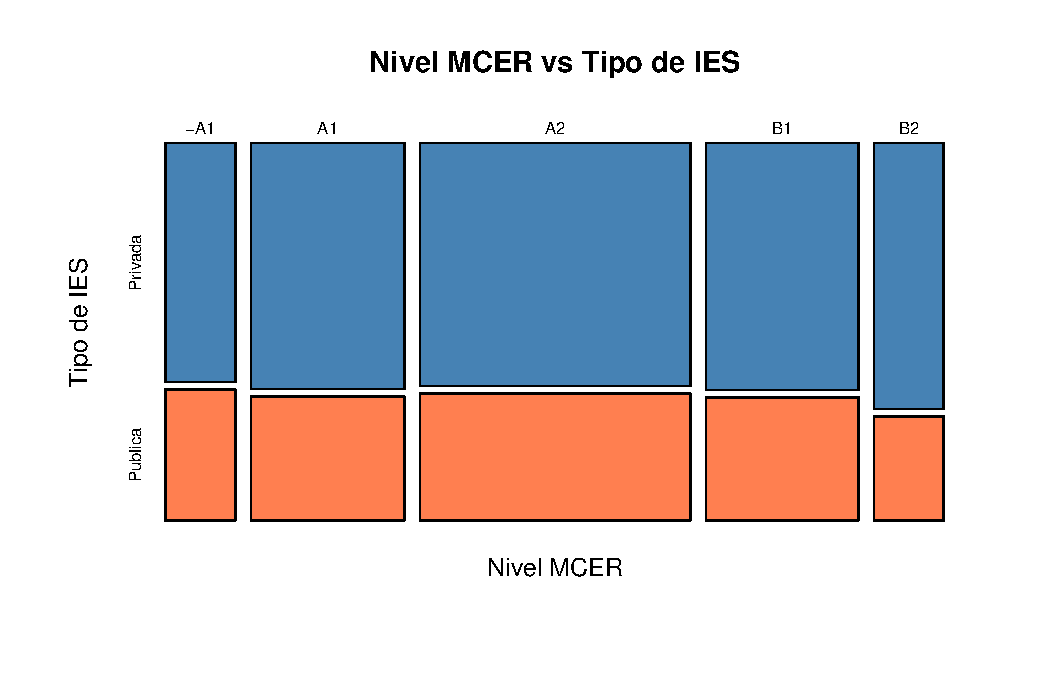
\includegraphics[width=0.85\textwidth]{figuras/mosaico.pdf}
\end{center}

\small Las IES privadas tienen \textbf{más} estudiantes en B1 y B2 de lo esperado y \textbf{menos} en $-$A1 y A1.
\end{frame}

% --- BONDAD DE AJUSTE ---

\begin{frame}[fragile]{Bondad de ajuste: ¿los niveles MCER son uniformes?}
\small
La prueba de \textbf{bondad de ajuste} compara una variable contra una distribución teórica.

\vspace{0.1cm}
$H_0$: Los 5 niveles MCER se distribuyen uniformemente. $H_1$: No.

\vspace{0.1cm}
\begin{lstlisting}[basicstyle=\ttfamily\scriptsize]
niveles <- table(saber_pro$MOD_INGLES_DESEM)
#  -A1   A1   A2   B1   B2
#  557 1278 1648 1007  595

chisq.test(niveles, p = rep(1/5, 5))
# X-squared = 841.76, df = 4, p-value < 2.2e-16
\end{lstlisting}

\vspace{0.1cm}
Rechazamos $H_0$: la distribución \textbf{no} es uniforme.

\vspace{0.1cm}
\begin{exampleblock}{Dos pruebas, misma fórmula}
\small
\textbf{Independencia}: ¿están asociadas dos variables? (tabla $r \times c$, gl $= (r{-}1)(c{-}1)$)\\
\textbf{Bondad de ajuste}: ¿esta variable sigue la distribución X? (un vector, gl $= k{-}1$)
\end{exampleblock}
\end{frame}

\begin{frame}{Distribución de niveles MCER}
\begin{center}
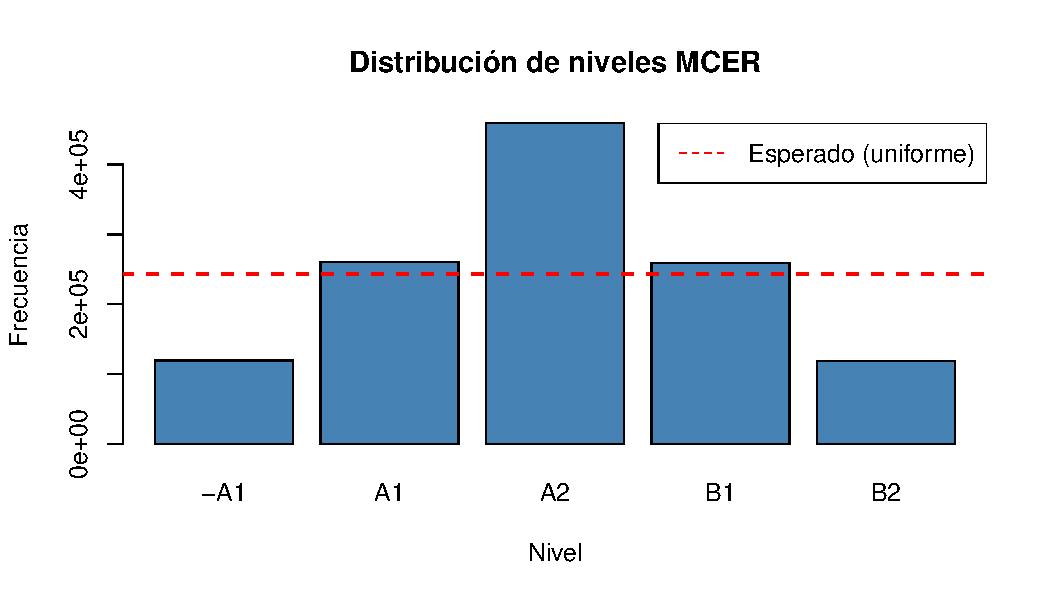
\includegraphics[width=0.8\textwidth]{figuras/barplot_mcer.pdf}
\end{center}

\small La línea roja punteada muestra la frecuencia esperada bajo uniformidad. Claro pico en A2 y baja frecuencia en los extremos.
\end{frame}

% --- TRANSICIÓN A SESIÓN 9 ---

\begin{frame}{¿Y cuando $Y$ es numérica?}
\begin{alertblock}{Limitación de $\chi^2$}
\small
Chi-cuadrado funciona cuando \textbf{ambas} variables son categóricas. Pero muchas preguntas en economía involucran variables numéricas: puntajes, salarios, precios.
\end{alertblock}

\vspace{0.3cm}
\begin{block}{Siguiente paso: regresión lineal}
¿Cuánto cambia el puntaje de inglés en Saber Pro por cada punto adicional en matemáticas de Saber 11? Necesitamos una herramienta que \textbf{cuantifique} relaciones entre variables numéricas.
\end{block}
\end{frame}

% ============================================================================
% SESIÓN 9: REGRESIÓN LINEAL SIMPLE (OLS)
% ============================================================================

\begin{frame}{}
\vfill
\centering
{\Large\textbf{Sesión 9}}\\[1em]
{\normalsize Regresión Lineal Simple (OLS)}\\[0.5em]
{\small El método de mínimos cuadrados ordinarios}
\vfill
\end{frame}

% ============================================================================
\section{Introducción a la regresión}
% ============================================================================

\begin{frame}{¿Por qué OLS es la herramienta central?}
\begin{exampleblock}{Porque todo en economía se reduce a OLS}
\small
\begin{itemize}\setlength{\itemsep}{2pt}
  \item Comparar grupos en sesiones anteriores: \textbf{era OLS} con dummies
  \item Rappi estima tiempos de entrega según distancia: OLS con $X$ continua
  \item Un banco modela riesgo crediticio: OLS con múltiples regresores
  \item Mincer estimó retornos a la educación: $\ln(\text{salario}) = \beta_0 + \beta_1 \cdot \text{años\_edu} + \varepsilon$
  \item En cualquier artículo de economía van a ver tablas de regresión --- es el idioma universal
\end{itemize}
\end{exampleblock}

\begin{alertblock}{Diferencia clave con correlación}
\small
La correlación les dice ``hay relación''. OLS les dice ``por cada punto más en Saber 11, esperamos $\hat{\beta}_1$ puntos más en Saber Pro''. Es pasar de describir a \textbf{predecir y cuantificar}.
\end{alertblock}
\end{frame}

\begin{frame}{Motivación: más allá de la correlación}
\begin{block}{Hasta ahora}
Hemos estudiado la \textbf{correlación} $r$ entre dos variables numéricas, que mide la fuerza y dirección de la relación lineal.
\end{block}

\vspace{0.1cm}
\textbf{Limitaciones de la correlación:}
\begin{itemize}
  \item Solo mide asociación, no permite predecir
  \item Es simétrica: $\text{cor}(X,Y) = \text{cor}(Y,X)$
  \item No distingue variable dependiente de independiente
\end{itemize}

\vspace{0.1cm}
\begin{exampleblock}{Pregunta de investigación}
\small ¿ Podemos \textbf{predecir} el desempeño en inglés en Saber Pro a partir del puntaje de matemáticas en Saber 11? Necesitamos un \textbf{modelo de regresión}.

\smallskip
\textbf{Analogía:} Imaginen que quieren predecir su nota del parcial a partir de las horas de estudio. La regresión es la herramienta que les permite hacer esa predicción de forma sistemática.
\end{exampleblock}
\end{frame}

\begin{frame}{El modelo de regresión lineal simple}
\begin{block}{Definición}
El modelo de \textbf{regresión lineal simple} relaciona una variable dependiente $Y$ con una variable independiente $X$ mediante una línea recta:
\[
Y_i = \beta_0 + \beta_1 X_i + \varepsilon_i
\]
donde:
\begin{itemize}
  \item $Y_i$ = valor observado de la variable dependiente (respuesta)
  \item $X_i$ = valor de la variable independiente (predictor, regressor)
  \item $\beta_0$ = intercepto (valor de $Y$ cuando $X = 0$)
  \item $\beta_1$ = pendiente (cambio en $Y$ por cada unidad de cambio en $X$)
  \item $\varepsilon_i$ = error aleatorio (desviación del modelo)
\end{itemize}
\end{block}
\vspace{-2pt}
{\small \textbf{Interpretación:} $\beta_0$ y $\beta_1$ son \textbf{parámetros poblacionales} (desconocidos). Los estimaremos con $\hat{\beta}_0$ y $\hat{\beta}_1$ usando los datos.}
\end{frame}

\begin{frame}{Ecuación estimada y valores ajustados}
La \textbf{ecuación estimada} (fitted line) es:
\[
\hat{Y}_i = \hat{\beta}_0 + \hat{\beta}_1 X_i
\]

\vspace{0.1cm}
\begin{itemize}
  \item $\hat{Y}_i$ = valor \textbf{predicho} (ajustado) de $Y$ para la observación $i$
  \item $e_i = Y_i - \hat{Y}_i$ = \textbf{residuo} (error de predicción)
\end{itemize}

\vspace{0.1cm}
\begin{exampleblock}{Ejemplo}
Si $\hat{\beta}_0 = 76.8$ y $\hat{\beta}_1 = 1.46$, la ecuación es:
\[
\widehat{\text{MOD\_INGLES\_PUNT}} = 76.8 + 1.46 \times \text{PUNT\_MATEMATICAS}
\]

Para un estudiante con puntaje 60 en matemáticas Saber 11:
\[
\hat{Y} = 76.8 + 1.46 \times 60 = 76.8 + 87.6 = 164.4
\]

Si su puntaje real en Saber Pro es 170, el residuo es $e = 170 - 164.4 = 5.6$.
\end{exampleblock}
\end{frame}

\begin{frame}[fragile]{Preparar datos: cruzar Saber Pro + Saber 11}
\begin{lstlisting}[basicstyle=\ttfamily\scriptsize]
# Cargar y cruzar Saber Pro + Saber 11
library(arrow); library(dplyr); library(ggplot2)
gh <- paste0("https://raw.githubusercontent.com/",
  "polanco-jaime/Curso-Estadistica-2026-3/",
  "main/datos")
sp  <- read_parquet(paste0(gh, "/saber_pro/saber_pro.parquet"))
s11 <- read_parquet(paste0(gh, "/saber11/saber11.parquet"))
cr  <- read_parquet(paste0(gh, "/cruce/",
       "cruce_saber11_saberpro.parquet"))

saber_pro <- sp |>
  inner_join(cr, by = c("ESTU_CONSECUTIVO" =
    "estu_consecutivo_sbpro")) |>
  inner_join(s11 |> select(ESTU_CONSECUTIVO,
    PUNT_INGLES, PUNT_MATEMATICAS),
    by = c("estu_consecutivo_sb11" =
    "ESTU_CONSECUTIVO"))
\end{lstlisting}

\vspace{0.2cm}
\begin{block}{¿Por qué cruzar?}
\small \texttt{PUNT\_MATEMATICAS} y \texttt{PUNT\_INGLES} están en Saber 11, no en Saber Pro. La tabla de cruce conecta ambos exámenes por estudiante.
\end{block}
\end{frame}

\begin{frame}[fragile]{Scatter plot + línea de regresión}
\begin{lstlisting}
ggplot(saber_pro, aes(x = PUNT_MATEMATICAS,
                     y = MOD_INGLES_PUNT)) +
  geom_point(alpha = 0.3, color = "steelblue") +
  geom_smooth(method = "lm", se = TRUE, color = "red",
              fill = "pink", alpha = 0.2) +
  labs(title = "Matematicas Saber 11 vs Ingles Saber Pro",
       x = "Puntaje matematicas Saber 11",
       y = "Puntaje ingles Saber Pro") +
  theme_minimal()
\end{lstlisting}
\end{frame}

\begin{frame}{Resultado: Matemáticas Saber 11 vs Inglés Saber Pro}
\begin{center}
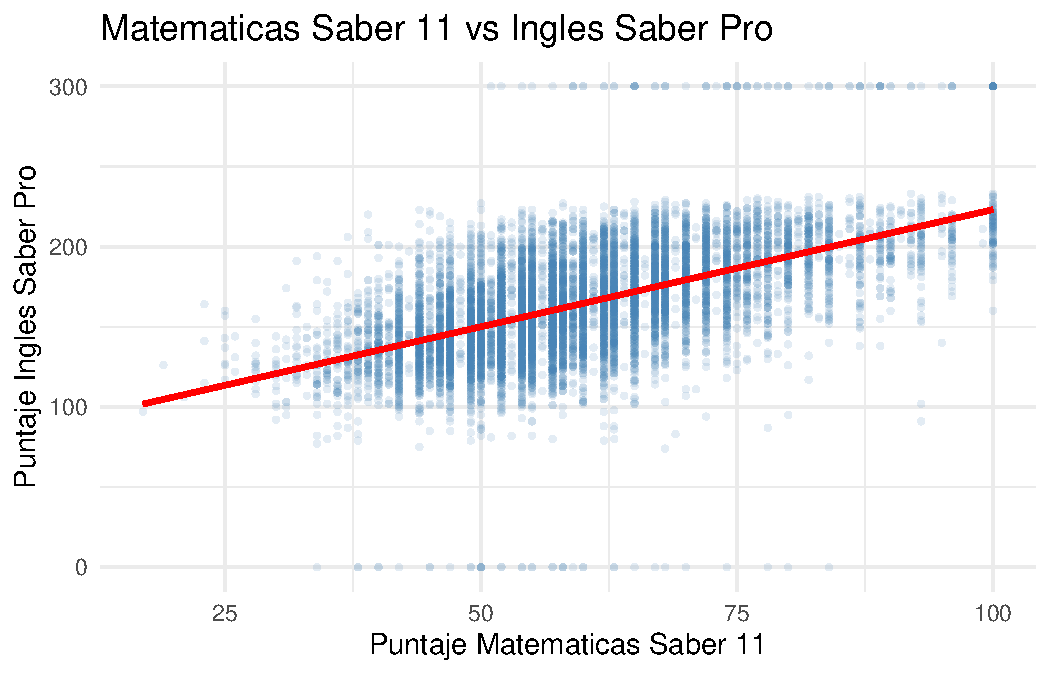
\includegraphics[width=0.85\textwidth]{figuras/scatter_modelo1.pdf}
\end{center}

\small La línea roja es la recta OLS. La banda rosada es el intervalo de confianza al 95\% para la media condicional $E(Y|X)$.
\end{frame}

\begin{frame}{¿Qué línea elegir?}
Hay infinitas líneas que pasan por la nube de puntos. ¿Cuál es la \textbf{mejor}?

\vspace{0.2cm}
\begin{block}{Criterio: minimizar los errores}
Queremos que los residuos $e_i = Y_i - \hat{Y}_i$ sean lo más pequeños posible en conjunto.
\end{block}

\vspace{0.2cm}
\textbf{Opciones:}
\begin{itemize}
  \item Minimizar $\sum |e_i|$ (suma de errores absolutos)
  \item Minimizar $\max |e_i|$ (error máximo)
  \item Minimizar $\sum e_i^2$ (suma de errores al cuadrado) $\leftarrow$ \textbf{OLS}
\end{itemize}
\end{frame}

\begin{frame}{Método de Mínimos Cuadrados Ordinarios (OLS)}
\begin{alertblock}{Definición}
El método \textbf{OLS} (Ordinary Least Squares) elige $\hat{\beta}_0$ y $\hat{\beta}_1$ que minimizan:
\[
\text{SSE} = \sum_{i=1}^{n} e_i^2 = \sum_{i=1}^{n} (Y_i - \hat{Y}_i)^2 = \sum_{i=1}^{n} (Y_i - \hat{\beta}_0 - \hat{\beta}_1 X_i)^2
\]
\end{alertblock}

\vspace{0.3cm}
En otras palabras: OLS busca la línea que minimiza los errores de predicción al cuadrado --- la línea que mejor ``le pega'' a los datos.
\end{frame}

% ============================================================================
\section{Método de mínimos cuadrados (OLS)}
% ============================================================================

\begin{frame}{¿Por qué entender cómo funciona OLS?}
\begin{exampleblock}{Porque necesitan leer y criticar tablas de regresión}
\small
\begin{itemize}\setlength{\itemsep}{2pt}
  \item Ya saben que OLS da la línea. Ahora necesitan entender \textbf{cómo la elige} y \textbf{cuándo confiar} en ella
  \item Cada artículo de economía tiene una tabla con coeficientes, errores estándar, $R^2$ y p-valores --- si no saben leerla, no pueden evaluar la evidencia
  \item Saber qué supuesto falla les dice si el modelo miente y cómo arreglarlo
\end{itemize}
\end{exampleblock}
\end{frame}

% --- POR QUE APRENDER LA DERIVACION -----------------------------------------

\begin{frame}{¿Por qué aprender la derivación y las matrices?}
\begin{exampleblock}{Porque sin esto, OLS es una caja negra}
\small
\begin{itemize}\setlength{\itemsep}{3pt}
  \item \texttt{lm()} les da números. Pero ¿de dónde salen? Si no entienden la fórmula, no pueden diagnosticar cuándo falla
  \item La notación matricial es el idioma de la econometría moderna: Wooldridge, Greene, Hayashi --- todos escriben $\hat{\boldsymbol{\beta}} = (\mathbf{X}'\mathbf{X})^{-1}\mathbf{X}'\mathbf{Y}$
  \item Con matrices, pasar de 1 regresor a 50 regresores es \textbf{cambiar el tamaño de $\mathbf{X}$}, nada más
  \item Entender la derivación les permite demostrar que OLS es insesgado: $E(\hat{\boldsymbol{\beta}}) = \boldsymbol{\beta}$
\end{itemize}
\end{exampleblock}

\begin{alertblock}{El plan}
\small Propiedades de $E(\cdot)$ $\to$ derivación escalar $\to$ notación matricial $\to$ ejemplo con 5 datos a mano $\to$ verificar en R.
\end{alertblock}
\end{frame}

% --- PROPIEDADES DE VALOR ESPERADO ------------------------------------------

\begin{frame}{Propiedades de valor esperado y varianza}
\small
\begin{block}{Valor esperado $E(\cdot)$}
\begin{enumerate}\setlength{\itemsep}{1pt}
  \item $E(c) = c$ \quad (constante)
  \item $E(cX) = cE(X)$ \quad (linealidad)
  \item $E(X + Y) = E(X) + E(Y)$ \quad (linealidad)
  \item $E(X - E(X)) = 0$ \quad (la media de las desviaciones es cero)
\end{enumerate}
\end{block}

\begin{block}{Varianza $\text{Var}(\cdot)$}
\begin{enumerate}\setlength{\itemsep}{1pt}
  \item $\text{Var}(c) = 0$
  \item $\text{Var}(cX) = c^2 \text{Var}(X)$
  \item $\text{Var}(X + Y) = \text{Var}(X) + \text{Var}(Y) + 2\text{Cov}(X,Y)$
  \item Si $X \perp Y$: $\text{Var}(X + Y) = \text{Var}(X) + \text{Var}(Y)$
\end{enumerate}
\end{block}

 
\end{frame}


\begin{frame}{Propiedades de valor esperado y varianza}
\small
 

\begin{alertblock}{Clave para OLS}
\small Bajo el modelo $Y_i = \beta_0 + \beta_1 X_i + \varepsilon_i$ con $E(\varepsilon_i | X_i) = 0$:
$E(Y_i | X_i) = \beta_0 + \beta_1 X_i$
\end{alertblock}
\end{frame}
% --- DERIVACION ESCALAR -----------------------------------------------------

\begin{frame}{Derivación escalar: ecuaciones normales}
\small
Minimizar $\text{SSE} = \sum_{i=1}^n (Y_i - \beta_0 - \beta_1 X_i)^2$. Derivadas parciales igualadas a cero:

\vspace{0.2cm}
\textbf{Respecto a $\beta_0$:}
\[
\frac{\partial \text{SSE}}{\partial \beta_0} = -2 \sum (Y_i - \beta_0 - \beta_1 X_i) = 0 \quad \Rightarrow \quad \sum Y_i = n\beta_0 + \beta_1 \sum X_i
\]

\textbf{Respecto a $\beta_1$:}
\[
\frac{\partial \text{SSE}}{\partial \beta_1} = -2 \sum X_i(Y_i - \beta_0 - \beta_1 X_i) = 0 \quad \Rightarrow \quad \sum X_i Y_i = \beta_0 \sum X_i + \beta_1 \sum X_i^2
\]

\vspace{0.2cm}
\textbf{Solución:}
\[
\boxed{\hat{\beta}_1 = \frac{\sum(X_i - \bar{X})(Y_i - \bar{Y})}{\sum(X_i - \bar{X})^2} = \frac{S_{XY}}{S_{XX}}} \qquad \boxed{\hat{\beta}_0 = \bar{Y} - \hat{\beta}_1 \bar{X}}
\]

La línea OLS \textbf{siempre} pasa por $(\bar{X}, \bar{Y})$.
\end{frame}

% --- INSESGADEZ EN VALOR ESPERADO -------------------------------------------

\begin{frame}{OLS es insesgado: $E(\hat{\beta}_1) = \beta_1$}
\small
\textbf{Demostrar que} $\hat{\beta}_1$ es un estimador insesgado de $\beta_1$:

\vspace{0.1cm}
Sustituimos $Y_i = \beta_0 + \beta_1 X_i + \varepsilon_i$ en la fórmula de $\hat{\beta}_1$:
\[
\hat{\beta}_1 = \frac{\sum(X_i - \bar{X})Y_i}{\sum(X_i - \bar{X})^2} = \frac{\sum(X_i - \bar{X})(\beta_0 + \beta_1 X_i + \varepsilon_i)}{S_{XX}}
\]

Expandiendo (y usando que $\sum(X_i - \bar{X}) = 0$ y $\sum(X_i - \bar{X})X_i = S_{XX}$):
\[
\hat{\beta}_1 = \frac{\cancel{\beta_0 \cdot 0} + \beta_1 S_{XX} + \sum(X_i - \bar{X})\varepsilon_i}{S_{XX}} = \beta_1 + \frac{\sum(X_i - \bar{X})\varepsilon_i}{S_{XX}}
\]

Tomando valor esperado condicional en $X$ y usando $E(\varepsilon_i | X_i) = 0$:
\[
E(\hat{\beta}_1 | \mathbf{X}) = \beta_1 + \frac{\sum(X_i - \bar{X}) \cdot 0}{S_{XX}} = \boxed{\beta_1}
\]

\begin{alertblock}{}
\small $\hat{\beta}_1$ es \textbf{insesgado}: en promedio, OLS acierta el verdadero $\beta_1$.
\end{alertblock}
\end{frame}

% --- DE ESCALARES A MATRICES ------------------------------------------------

\begin{frame}{De escalares a matrices: ¿por qué?}
\small

Con un solo regresor, las fórmulas escalares funcionan. Pero con $k$ regresores:
\[
Y_i = \beta_0 + \beta_1 X_{1i} + \beta_2 X_{2i} + \cdots + \beta_k X_{ki} + \varepsilon_i
\]

tendríamos $k+1$ ecuaciones normales. Las matrices lo simplifican a \textbf{una sola expresión}:

\vspace{0.2cm}
\begin{block}{Notación matricial del modelo}
\[
\underbrace{\mathbf{Y}}_{n \times 1} = \underbrace{\mathbf{X}}_{n \times (k+1)} \underbrace{\boldsymbol{\beta}}_{(k+1) \times 1} + \underbrace{\boldsymbol{\varepsilon}}_{n \times 1}
\]
\end{block}

donde $\mathbf{X}$ incluye una columna de unos para el intercepto:
\[
\mathbf{X} = \begin{pmatrix} 1 & X_{11} & \cdots & X_{k1} \\ 1 & X_{12} & \cdots & X_{k2} \\ \vdots & \vdots & \ddots & \vdots \\ 1 & X_{1n} & \cdots & X_{kn} \end{pmatrix}, \quad
\boldsymbol{\beta} = \begin{pmatrix} \beta_0 \\ \beta_1 \\ \vdots \\ \beta_k \end{pmatrix}, \quad
\mathbf{Y} = \begin{pmatrix} Y_1 \\ Y_2 \\ \vdots \\ Y_n \end{pmatrix}
\]
\end{frame}

% --- DERIVACION MATRICIAL ---------------------------------------------------

\begin{frame}{Derivación matricial de OLS}
\small
Minimizar $\text{SSE} = \boldsymbol{\varepsilon}'\boldsymbol{\varepsilon} = (\mathbf{Y} - \mathbf{X}\boldsymbol{\beta})'(\mathbf{Y} - \mathbf{X}\boldsymbol{\beta})$:

\vspace{0.1cm}
\textbf{Paso 1:} Expandir
\[
\text{SSE} = \mathbf{Y}'\mathbf{Y} - 2\boldsymbol{\beta}'\mathbf{X}'\mathbf{Y} + \boldsymbol{\beta}'\mathbf{X}'\mathbf{X}\boldsymbol{\beta}
\]

\textbf{Paso 2:} Derivar respecto a $\boldsymbol{\beta}$ e igualar a cero
\[
\frac{\partial \text{SSE}}{\partial \boldsymbol{\beta}} = -2\mathbf{X}'\mathbf{Y} + 2\mathbf{X}'\mathbf{X}\boldsymbol{\beta} = \mathbf{0}
\]

\textbf{Paso 3:} Resolver (ecuaciones normales en matrices)
\[
\mathbf{X}'\mathbf{X}\hat{\boldsymbol{\beta}} = \mathbf{X}'\mathbf{Y}
\]

\textbf{Paso 4:} Premultiplicar por $(\mathbf{X}'\mathbf{X})^{-1}$
\[
\boxed{\hat{\boldsymbol{\beta}} = (\mathbf{X}'\mathbf{X})^{-1}\mathbf{X}'\mathbf{Y}}
\]

\begin{alertblock}{}
\small Esta fórmula funciona para 1 regresor o 1000. Solo cambia el tamaño de $\mathbf{X}$.
\end{alertblock}
\end{frame}

% --- INSESGADEZ MATRICIAL ---------------------------------------------------

\begin{frame}{Insesgadez en notación matricial}
\small
Sustituimos $\mathbf{Y} = \mathbf{X}\boldsymbol{\beta} + \boldsymbol{\varepsilon}$ en $\hat{\boldsymbol{\beta}} = (\mathbf{X}'\mathbf{X})^{-1}\mathbf{X}'\mathbf{Y}$:

\begin{align*}
\hat{\boldsymbol{\beta}} &= (\mathbf{X}'\mathbf{X})^{-1}\mathbf{X}'(\mathbf{X}\boldsymbol{\beta} + \boldsymbol{\varepsilon}) \\
&= \underbrace{(\mathbf{X}'\mathbf{X})^{-1}\mathbf{X}'\mathbf{X}}_{\mathbf{I}}\boldsymbol{\beta} + (\mathbf{X}'\mathbf{X})^{-1}\mathbf{X}'\boldsymbol{\varepsilon} \\
&= \boldsymbol{\beta} + (\mathbf{X}'\mathbf{X})^{-1}\mathbf{X}'\boldsymbol{\varepsilon}
\end{align*}

Tomando valor esperado condicional en $\mathbf{X}$ y usando $E(\boldsymbol{\varepsilon} | \mathbf{X}) = \mathbf{0}$:
\[
E(\hat{\boldsymbol{\beta}} | \mathbf{X}) = \boldsymbol{\beta} + (\mathbf{X}'\mathbf{X})^{-1}\mathbf{X}' \cdot \mathbf{0} = \boxed{\boldsymbol{\beta}}
\]

\begin{block}{Varianza de $\hat{\boldsymbol{\beta}}$}
Si además $\text{Var}(\boldsymbol{\varepsilon} | \mathbf{X}) = \sigma^2 \mathbf{I}$ (homocedasticidad):
\[
\text{Var}(\hat{\boldsymbol{\beta}} | \mathbf{X}) = \sigma^2 (\mathbf{X}'\mathbf{X})^{-1}
\]
Los errores estándar de la tabla de \texttt{summary()} salen de la diagonal de esta matriz.
\end{block}
\end{frame}

% --- EJEMPLO CON 5 DATOS ---------------------------------------------------

\begin{frame}{Ejemplo a mano: 5 estudiantes}
\small
\textbf{Pregunta:} ¿Cuántos puntos más de inglés (Saber Pro) esperamos por cada punto adicional en matemáticas (Saber 11)?

\vspace{0.2cm}
\begin{center}
\begin{tabular}{ccc}
\toprule
Estudiante $i$ & Matemáticas ($X_i$) & Inglés ($Y_i$) \\
\midrule
1 & 40 & 130 \\
2 & 50 & 145 \\
3 & 60 & 160 \\
4 & 70 & 175 \\
5 & 80 & 200 \\
\midrule
& $\bar{X} = 60$ & $\bar{Y} = 162$ \\
\bottomrule
\end{tabular}
\end{center}

\vspace{0.2cm}
\textbf{Modelo:} $Y_i = \beta_0 + \beta_1 X_i + \varepsilon_i$

Vamos a estimar $\hat{\boldsymbol{\beta}}$ de tres formas: fórmula escalar, fórmula matricial, y \texttt{lm()} en R.
\end{frame}

% --- PASO 1: FORMULA ESCALAR -----------------------------------------------

\begin{frame}{Paso 1: fórmula escalar}
\small
\[
\hat{\beta}_1 = \frac{S_{XY}}{S_{XX}} = \frac{\sum(X_i - \bar{X})(Y_i - \bar{Y})}{\sum(X_i - \bar{X})^2}
\]

\begin{center}
\footnotesize
\begin{tabular}{crrrrr}
\toprule
$i$ & $X_i$ & $Y_i$ & $X_i - 60$ & $Y_i - 162$ & $(X_i{-}60)(Y_i{-}162)$ \\
\midrule
1 & 40 & 130 & $-20$ & $-32$ & 640 \\
2 & 50 & 145 & $-10$ & $-17$ & 170 \\
3 & 60 & 160 & 0 & $-2$ & 0 \\
4 & 70 & 175 & 10 & 13 & 130 \\
5 & 80 & 200 & 20 & 38 & 760 \\
\midrule
& & & & $S_{XY} =$ & \textbf{1700} \\
\bottomrule
\end{tabular}
\end{center}

$S_{XX} = (-20)^2 + (-10)^2 + 0^2 + 10^2 + 20^2 = 400 + 100 + 0 + 100 + 400 = \mathbf{1000}$

\[
\hat{\beta}_1 = \frac{1700}{1000} = \mathbf{1.70} \qquad \hat{\beta}_0 = 162 - 1.70 \times 60 = \mathbf{60}
\]

$\hat{Y} = 60 + 1.70 X$: por cada punto más en matemáticas, 1.70 puntos más en inglés.
\end{frame}

% --- PASO 2: ARMAR MATRICES ------------------------------------------------

\begin{frame}{Paso 2: armar $\mathbf{X}$ e $\mathbf{Y}$}
Agregamos la columna de unos para el intercepto:

\[
\mathbf{X} = \begin{pmatrix} 1 & 40 \\ 1 & 50 \\ 1 & 60 \\ 1 & 70 \\ 1 & 80 \end{pmatrix}_{5 \times 2}
\qquad
\mathbf{Y} = \begin{pmatrix} 130 \\ 145 \\ 160 \\ 175 \\ 200 \end{pmatrix}_{5 \times 1}
\qquad
\boldsymbol{\beta} = \begin{pmatrix} \beta_0 \\ \beta_1 \end{pmatrix}_{2 \times 1}
\]

\vspace{0.3cm}
\textbf{Verificar dimensiones:}
\[
\underbrace{\mathbf{Y}}_{5\times 1} = \underbrace{\mathbf{X}}_{5\times 2} \underbrace{\boldsymbol{\beta}}_{2\times 1} + \underbrace{\boldsymbol{\varepsilon}}_{5\times 1} \quad \checkmark
\]

\begin{exampleblock}{Regla práctica}
$\mathbf{X}$ siempre tiene $n$ filas (observaciones) y $k+1$ columnas (intercepto + $k$ regresores).
\end{exampleblock}
\end{frame}

% --- PASO 3: CALCULAR X'X y X'Y -------------------------------------------

\begin{frame}{Paso 3: calcular $\mathbf{X}'\mathbf{X}$ y $\mathbf{X}'\mathbf{Y}$}
\small
\[
\mathbf{X}'\mathbf{X} = \begin{pmatrix} 1&1&1&1&1 \\ 40&50&60&70&80 \end{pmatrix} \begin{pmatrix} 1&40 \\ 1&50 \\ 1&60 \\ 1&70 \\ 1&80 \end{pmatrix} = \begin{pmatrix} 5 & 300 \\ 300 & 19000 \end{pmatrix}
\]

\[
\mathbf{X}'\mathbf{Y} = \begin{pmatrix} 1&1&1&1&1 \\ 40&50&60&70&80 \end{pmatrix} \begin{pmatrix} 130 \\ 145 \\ 160 \\ 175 \\ 200 \end{pmatrix} = \begin{pmatrix} 810 \\ 50300 \end{pmatrix}
\]

\vspace{0.2cm}
\textbf{Interpretación de $\mathbf{X}'\mathbf{X}$:}
\begin{itemize}\setlength{\itemsep}{0pt}
  \item Esquina superior izquierda: $n = 5$
  \item Esquina superior derecha: $\sum X_i = 300$
  \item Esquina inferior derecha: $\sum X_i^2 = 19000$
\end{itemize}
\end{frame}

% --- PASO 4: INVERTIR X'X -------------------------------------------------

\begin{frame}{Paso 4: invertir $(\mathbf{X}'\mathbf{X})^{-1}$}
\small
Para una matriz $2 \times 2$: $\begin{pmatrix} a & b \\ c & d \end{pmatrix}^{-1} = \frac{1}{ad - bc}\begin{pmatrix} d & -b \\ -c & a \end{pmatrix}$

\vspace{0.2cm}
\[
\text{det} = 5 \times 19000 - 300 \times 300 = 95000 - 90000 = 5000
\]

\[
(\mathbf{X}'\mathbf{X})^{-1} = \frac{1}{5000}\begin{pmatrix} 19000 & -300 \\ -300 & 5 \end{pmatrix} = \begin{pmatrix} 3.80 & -0.06 \\ -0.06 & 0.001 \end{pmatrix}
\]

\vspace{0.2cm}
\begin{alertblock}{Ahora aplicar la fórmula}
\[
\hat{\boldsymbol{\beta}} = (\mathbf{X}'\mathbf{X})^{-1}\mathbf{X}'\mathbf{Y} = \begin{pmatrix} 3.80 & -0.06 \\ -0.06 & 0.001 \end{pmatrix} \begin{pmatrix} 810 \\ 50300 \end{pmatrix}
\]
\[
= \begin{pmatrix} 3078 - 3018 \\ -48.6 + 50.3 \end{pmatrix} = \boxed{\begin{pmatrix} 60 \\ 1.70 \end{pmatrix}}
\]
\end{alertblock}

$\hat{\beta}_0 = 60$, $\hat{\beta}_1 = 1.70$ --- \textbf{idéntico} al resultado escalar. $\checkmark$
\end{frame}

% --- PASO 5: EN R ----------------------------------------------------------

\begin{frame}[fragile]{Paso 5: verificar en R}
\begin{lstlisting}[basicstyle=\ttfamily\scriptsize]
# Los 5 datos
X_val <- c(40, 50, 60, 70, 80)
Y_val <- c(130, 145, 160, 175, 200)

# --- Forma matricial ---
X <- cbind(1, X_val)      # agregar columna de unos
Y <- matrix(Y_val, ncol = 1)

beta_hat <- solve(t(X) %*% X) %*% t(X) %*% Y
beta_hat

#      [,1]
# [1,] 60.0
# [2,]  1.7

# --- Con lm() ---
modelo <- lm(Y_val ~ X_val)
coef(modelo)

# (Intercept)       X_val
#        60.0         1.7
\end{lstlisting}

\begin{block}{}
\small Tres caminos, mismo resultado: fórmula escalar, $(\mathbf{X}'\mathbf{X})^{-1}\mathbf{X}'\mathbf{Y}$, y \texttt{lm()}. \texttt{lm()} internamente usa una descomposición QR (más estable numéricamente), pero el resultado es el mismo.
\end{block}
\end{frame}

% --- RELACION CON CORRELACION -----------------------------------------------

\begin{frame}{Relación con la correlación}
El estimador OLS de la pendiente se puede escribir como:
\[
\hat{\beta}_1 = r \times \frac{s_Y}{s_X}
\]
\begin{small}
donde $r$ = correlación de Pearson, $s_Y$ = desviación estándar de $Y$, $s_X$ = desviación estándar de $X$.
\end{small}

\vspace{0.2cm}
\textbf{Interpretación:}
\begin{itemize}
  \item Si $r = 0$ $\Rightarrow$ $\hat{\beta}_1 = 0$ (no hay relación lineal)
  \item Si $s_X = s_Y$ y $r = 1$ $\Rightarrow$ $\hat{\beta}_1 = 1$ (relación 1 a 1)
  \item El signo de $\hat{\beta}_1$ es el mismo que el de $r$
\end{itemize}

\vspace{0.1cm}
\begin{exampleblock}{Verificar con nuestro ejemplo}
\small $r = 0.993$, $s_X = 15.81$, $s_Y = 26.93$. Entonces $\hat{\beta}_1 = 0.993 \times \frac{26.93}{15.81} = 0.993 \times 1.703 = 1.70$ $\checkmark$
\end{exampleblock}
\end{frame}

\begin{frame}[fragile]{Aplicación en R: \texttt{lm()}}
\begin{lstlisting}[basicstyle=\ttfamily\scriptsize]
# Ajustar modelo de regresion lineal simple
modelo1 <- lm(MOD_INGLES_PUNT ~ PUNT_MATEMATICAS,
              data = saber_pro)

# Ver coeficientes estimados
coef(modelo1)

#      (Intercept) PUNT_MATEMATICAS
#            76.78             1.46

# Interpretar
# beta_0 = 76.78: puntaje esperado en ingles Saber Pro
#                 si matematicas Saber 11 = 0
# beta_1 = 1.46: por cada punto adicional en matematicas,
#                esperamos 1.46 puntos mas en ingles
\end{lstlisting}

\vspace{0.2cm}
\begin{alertblock}{Cuidado con la extrapolación}
$\hat{\beta}_0 = 76.78$ representa el intercepto teórico, pero en la práctica nadie obtiene 0 en matemáticas. No interprete el intercepto fuera del rango de los datos.
\end{alertblock}
\end{frame}

\begin{frame}[fragile]{Valores ajustados y residuos}
\begin{lstlisting}[basicstyle=\ttfamily\scriptsize,aboveskip=0pt,belowskip=0pt]
# Valores ajustados (predicciones)
y_hat <- fitted(modelo1)
head(y_hat)

# 186.4 192.2 176.2 168.9 171.8 182.0 ...

# Residuos
residuos <- residuals(modelo1)
head(residuos)

# 12.6 22.8 -5.2 3.1 40.2 11.0 ...

# Verificar: la suma de residuos es (casi) 0
sum(residuos)

# [1] -1.6e-08  (numericamente 0)

# Verificar: la correlacion entre X y residuos es (casi) 0
cor(saber_pro$PUNT_MATEMATICAS, residuos)

# [1] -3.5e-17  (numericamente 0)
\end{lstlisting}

{\small \textbf{Propiedades OLS:} $\sum e_i = 0$ y $\sum X_i e_i = 0$ (ortogonalidad).}
\end{frame}

\begin{frame}[fragile]{Visualización de residuos}
\begin{lstlisting}
# Grafico de residuos vs valores ajustados
plot(fitted(modelo1), residuals(modelo1),
     xlab = "Valores ajustados",
     ylab = "Residuos",
     main = "Residuos vs Valores Ajustados",
     pch = 20, col = "steelblue")
abline(h = 0, col = "red", lwd = 2, lty = 2)

# Idealmente, los residuos deberian estar dispersos
# aleatoriamente alrededor de 0, sin patron visible
\end{lstlisting}

\vspace{0.2cm}
\begin{block}{Diagnóstico}
\begin{itemize}
  \item Patrón en forma de embudo $\Rightarrow$ heterocedasticidad
  \item Patrón curvo $\Rightarrow$ no linealidad
  \item Dispersión aleatoria $\Rightarrow$ supuestos plausibles
\end{itemize}
\end{block}
\end{frame}

\begin{frame}{Resultado: residuos vs valores ajustados}
\begin{center}
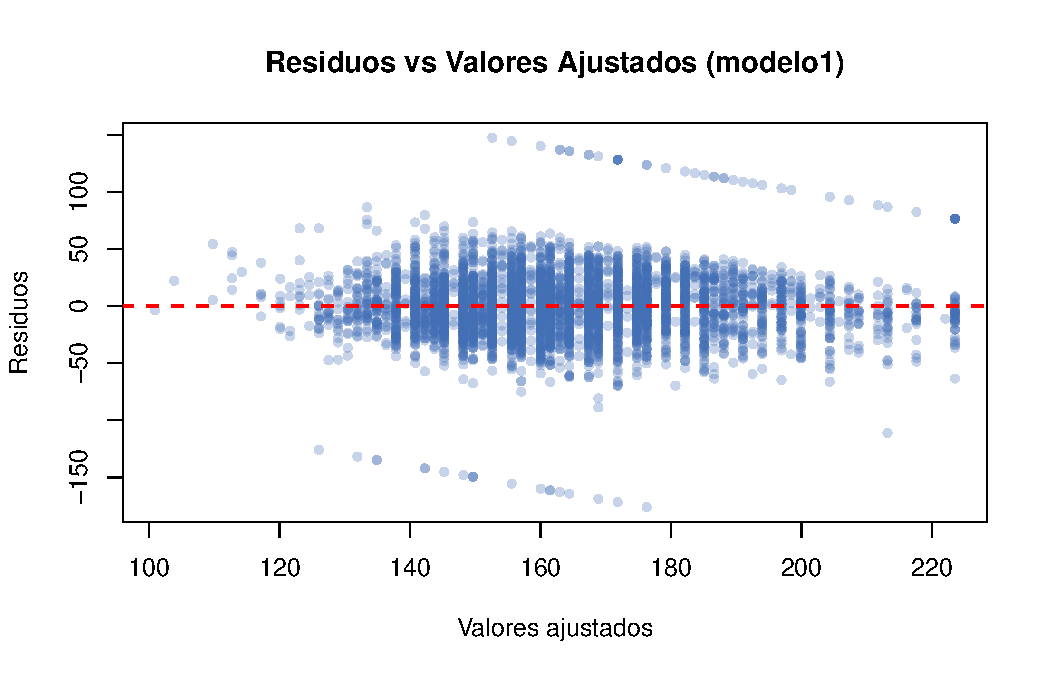
\includegraphics[width=0.85\textwidth]{figuras/residuos_modelo1.pdf}
\end{center}

\small Se observa dispersión relativamente uniforme alrededor de 0, aunque con algo de estructura en los extremos. Los supuestos parecen razonables, pero verificaremos formalmente en la próxima sesión.
\end{frame}

\begin{frame}{Próxima sesión (S09)}
\begin{block}{Lo que viene}
\begin{itemize}\setlength{\itemsep}{3pt}
  \item \textbf{Supuestos de Gauss-Markov}: ¿cuándo confiar en OLS y cuándo no?
  \item \textbf{$R^2$}: ¿qué tan bueno es nuestro modelo?
  \item \textbf{Pruebas de significancia}: ¿$\hat{\beta}_1$ es real o casualidad?
  \item \textbf{Variables dummy y multicolinealidad}: comparar grupos con OLS
  \item \textbf{Ejemplos de investigación real}: tablas de regresión en artículos de economía
\end{itemize}
\end{block}
\end{frame}

\begin{frame}
\begin{center}
\Large
¡Gracias por su atención!

\vspace{1cm}
\normalsize
Preguntas y discusión
\end{center}
\end{frame}

\end{document}
